% File: project_notebook.tex
% Description: TeX file to generate Project Notebook (template)
% Author: George Hadley
% Website: http://nbitwonder.com
% Notes:
% 1) This document is written using the LaTeX typesetting language. For more information on
%	LaTeX, consult http://en.wikibooks.org/wiki/LaTeX/
% 2) This document needs to be compiled using pdfLaTeX. It is not supported with pdfTeX
%	at the present time
% 3) This document utilizes the \nbwheader command created in doc_header.tex. By default,
%	this file is located at:
%	/path-to-documentation-templates/lbr/doc_header.tex
% 4) This document utilizes commands and environments created in projnb_lbr.tex. By default,
%	this file is located at:
%	/path-to-documentation-templates/lbr/projnb_lbr.tex
% Version: 0.1
% Last Modified: 1-04-2010
\documentclass[12pt,letterpaper,onecolumn]{article}
\usepackage{graphicx}
\usepackage{float}
\usepackage{subfig}
\usepackage{tikz}
\usepackage{fancyhdr}
\usepackage{verbatim}
\usepackage{kpfonts}
\usepackage{fullpage}
\usepackage{hyperref}

%Page layout settings
\setlength{\voffset}{-10pt}
\setlength{\headsep}{20pt}
\setlength{\headheight}{15pt}
\setlength{\topmargin}{-20pt}

%Path to open documentation system global lbr directory
%Set to /path-to-documentation-templates/lbr
%\newcommand{\globallbr}{/Users/georgehadley/Documents/NBitWonder/IT/Tools/ProjectTemplates/lbr}
\newcommand{\globallbr}{../lbr}

\begin{comment}
  Hyperref settings: settings for the hyperref hyperlink package.
  For a more detailed listing of available settings, consult 
  	http://en.wikibooks.org/wiki/LaTeX/Hyperlinks#Customization

  IMPORTANT: For your document, modify the pdftitle, pdfauthor, pdfsubject,
	and pdfkeywords options to tailor to your document
\end{comment}
\hypersetup{
	bookmarks=true, 					%Enable pdf bookmarks
	pdfborder={0,0,0},					%Disable borders around links
	pdftitle={Project Notebook (template)},		%Name of PDF document
	pdfauthor={George Hadley},				%Author of PDF document
	pdfsubject={Embedded Electronics},		%Subject of PDF document
	pdfkeywords={diy,electronics,nbitwonder},	%Keywords for PDF document
	colorlinks={true},					%Enable colored links
	linkcolor=red,						%Internal link color
	citecolor=green,						%Citation link color
	filecolor=blue,						%File link color
	urlcolor=blue						%URL link color
}


% File: doc_header.tex
% Description: TeX command used to develop custom documentation header used in Open
%	 Documentation System
% Author: George Hadley
% Website: http://nbitwonder.com
% Notes: 
% 	1) Derived from LaTeX example 'TeXblog: Fancy chapter headings with TikZ' found at
%		http://texblog.net/latex-archive/layout/fancy-chapter-tikz/
%	2) For additional help with the LaTeX package, consult the WikiBook found at
%		http://en.wikibooks.org/wiki/LaTeX
%	3) This file needs to be compiled with pdfLaTeX (does not appear to be compatible with
%		pdfTeX at the present time)
% Version: 0.1
% Last Modified: 12-28-2010

%Variable Declarations (modify these to tweak the header on your document)
\newcommand{\headery}{-3cm}					%y-offset of header (bottom left corner of header)
\newcommand{\headercolor}{black}				%Background color of header
\newcommand{\headerxstart}{.1\paperwidth}			%Starting x-coordinate for header box
\newcommand{\headerystart}{0cm}				%Starting y-coordinate for header box
\newcommand{\headerxend}{.9\paperwidth}			%Ending x-coordinate for header box
\newcommand{\headeryend}{2cm}				%Ending y-coordinate for header box
\newcommand{\logoxstart}{.1\paperwidth}			%Starting x-coordinate for logo
\newcommand{\logoystart}{1cm}					%Starting y-coordinate for logo
\newcommand{\logolink}{http://nbitwonder.com}		%URL for website, etc.
\newcommand{\logoheight}{40pt}					%Height of logo image
\newcommand{\logoloc}{../lbr/img/NBitWonderLogo_wTm.png}	%Path to logo image
\newcommand{\docboxxstart}{.5\paperwidth}		%Starting x-coordinate of documentation box
\newcommand{\docboxystart}{1cm}				%Starting y-coordinate of documentation box
\newcommand{\docboxwidth}{.38\paperwidth}		%Width of documentation box
\newcommand{\docboxtextcolor}{green}			%Text color in documentation box

% Command: \nbwheader
% Description: Creates a documentation header for use in the Open Documentation System templates
% Usage: \nbwheader{DocumentName}{ProjectName}{ProjectVersion} where
%	DocumentName is the name of the document (e.g. Project Notebook, User Manual, Bug Tracker, etc.
%	ProjectName is the name of the project the documentation is about
%	ProjectVersion is the current version of the project
\newcommand{\nbwheader}[3]
{
    \begin{tikzpicture}[remember picture,overlay]
    \node[yshift=\headery] at (current page.north west)
    {
        \begin{tikzpicture}[remember picture, overlay]
        \draw[fill=\headercolor] (\headerxstart,\headerystart) rectangle
            (\headerxend,\headeryend);
        \node[anchor=west,xshift=\logoxstart,yshift=\logoystart,rectangle]
        {\href{\logolink}{\includegraphics[height=\logoheight]{\logoloc}}};
        \node[anchor=west,xshift =\docboxxstart,yshift=\docboxystart,rectangle]
        {
            \begin{minipage}{\docboxwidth}
	   \begin{flushright}
	   \normalsize\textcolor{\docboxtextcolor}{\textsc{
	   \linespread{2}
	   #1 \\
	   Project: #2 \\
	   Version: #3 \\
            }}
	   \end{flushright}
            \end{minipage}};
        \end{tikzpicture}
        };
    \end{tikzpicture}
}

% File: aliases.tex
% Description: TeX library aliases used in open documentation templates
% Author: George Hadley
% Website: http://nbitwonder.com
% Notes: 
%	1) For additional help with the LaTeX package, consult the WikiBook found at
%		http://en.wikibooks.org/wiki/LaTeX
%	2) This file needs to be compiled with pdfLaTeX (does not appear to be compatible with
%		pdfTeX at the present time)
% Version: 0.1
% Last Modified: 1-04-2010
\newcommand{\ohm}{$\Omega$}
\newcommand{\uF}{$\mu$F}
% File: project_notebook_lbr.tex
% Description: TeX commands used for the project notebook in the Open 
%	Documentation System
% Author: George Hadley
% Website: http://nbitwonder.com
% Notes:
% 1) This document was written using the LaTeX typesetting language. For more help
%	with the LaTeX typesetting language, consult: http://en.wikibooks.org/wiki/LaTeX/
% 2) This file needs to be compiled with pdfLaTeX (does not appear to be compatible with
%	pdfTeX at the present time
% Version: 0.0
% Last Modified: 12-28-2010

% Variable Declarations: \projnbtagline command

% Command: \projnbtagline
% Description: Creates a tagline for use in the Project Notebook entries
% Usage: \projnbtagline{Entry#}{Date}{Version}{Title} where
% 	Entry# is the number of the current entry
%	Date is the date of the current entry
%	Version is the version number of the current entry (major and minor version)
%	Title is a short, descriptive title of the project entry
\newcommand{\projnbtagline}[4]
{
\textbf{Entry:} #1 \textbf{Date:} #2 \textbf{Version:} #3 \textbf{Title:} #4
\hfill
}

%Variable declarations: \nbentry environment

% Environment: nbentry
% Description: Environment defined for project notebook entries
% Usage: \begin{nbentry}{Entry#}{Date}{Version}{Title} where
% 	Entry# is the number of the current entry
%	Date is the date of the current entry
%	Version is the version number of the current entry (major and minor version)
%	Title is a short, descriptive title of the project entry

\newenvironment{nbentry}[4]
{\noindent\\\framebox{\projnbtagline{#1}{#2}{#3}{#4}}\\}
{}


%Modify these to reflect your documentation
\newcommand{\documentationtype}{Project Notebook}
\newcommand{\projectname}{RGBSaber }
\newcommand{\projectversion}{1}

%Header/Footer Definitions
\pagestyle{fancy}
\lhead{ }
\chead{ }
\rhead{\projectname  v\projectversion \documentationtype}
\lfoot{\href{http://nbitwonder.com}{http://nbitwonder.com} }
\cfoot{\thepage}
\rfoot{\copyright 2011 NBitWonder, LLC }

\begin{document}
\thispagestyle{plain}
% Insert title page or header here
\nbwheader{\documentationtype}{\projectname}{\projectversion}
% Insert optional project index here
% For long projects, it is recommended that project entries be indexed
%	by entry, week, month, or year (or a combination of the above)

% Project Notebook entries
% Project Notebook entries should be enclosed in boxes and contain a tagline
%	detailing the entry number, date, revision (project minor version), and 
%	a short, descriptive title
\begin{nbentry}{001}{8/22/2010}{1.4}{v1.5 Redesign}
\indent This past weekend I once again attempted to construct the RGB Lightsaber, using the chassis I had ordered from the Custom Saber Shop. Unfortunately, an unknown internal short occurred within this lightsaber, destroying the control board. This and other problems have forced me to redesign the RGB driver board, resulting in RGBSaber v1.5. A list of changes to be made in v1.5 include the following:
\begin{enumerate}
\item Change power source from 6-AA NiMH batteries to 2-cell 7.4V Li-Ion pack. In making this change, undervoltage protection must be included in Li-Ion pack to prevent damage to the batteries.
\item Flip power converter unit to top-side of the board. The lithium ion protection circuitry may be placed on the bottom of the board.
\item Move RGB led connector from top edge of board to the right side of the board to ease connection issues.
\item Use connectors for all interfaces, to maximize reuse and increase reliability (solder makes for poor electrical connections).
\item Minimize wiring inside of lightsaber chassis. Try to limit wire lengths to 3 inches or less.
\end{enumerate}
\end{nbentry}

\begin{nbentry}{002}{8/26/2010}{1.5}{v1.5 Connectors}
\indent Today I am performing redesign work on the RGB Lightsaber, designing and laying out RGBSaber v1.5. In order to get the saber up and running, reliable connectors are required for the design. As such, today's entry details the search for good connectors to use on the RGB Lightsaber project. \\
\indent To begin the search, I went to \href{http://www.molex.com/}{Molex} and began looking at the connector options they had, with hopes of getting free samples of some of the connectors. Promising connectors included the PicoBlade connectors for the peripheral board connection. Unfortunately, after additional searching, it was determined that the crimping tools needed for the PicoBlade connectors were prohibitively expensive (hundreds of dollars) and cable subassemblies did not appear to be available.
\end{nbentry}

\begin{nbentry}{003}{8/27/2010}{1.5}{v1.5 Undervoltage Protection}
\indent Following yesterday's connector search, I continued the search for reliable, feasible connectors to use for the RGBSaber project. Leaving Molex and looking for connector possibilities over at \href{http://tycoelectronics.com}{Tyco Electronics}, I found some additional promising possibilities. Particularly promising were the \href{http://www.tycoelectronics.com/catalog/feat/en/c/11398?BML=10576,17560,23645,17587}{Micro-MaTch} and \href{http://www.tycoelectronics.com/catalog/feat/en/s/23478?BML=10576,17560,23645,17587}{MTA100} connectors. More promising still, a crimping tool was available for these connectors at a very reasonable price of 18 dollars. \\
\indent Having found a reasonable connector option for the board, I proceded to investigate undervoltage protection options for the lightsaber power circuitry. In order to meet acceptable size requirements, v1.5 of the RGBSaber circuitry is to be powered by a 2-cell 7.4V Li-Ion battery pack. To prevent damage to the Li-Ion pack, a simple analog circuit will be designed to kill power to the circuit in the event that the battery pack voltage drops below 5.6V (signifying an undervoltage condition).
\end{nbentry}

\begin{nbentry}{004}{9/01/2010}{1.5}{v1.5 Undervoltage Protection 2}
\indent Research continued on the Li-Ion undervoltage protection circuit. Comparator circuits were investigated for their use within the RGBSaber control circuit. I was hoping to utilize a comparator with an integrated voltage reference, however, these were shown to be prohibitively expensive. Therefore, a general purpose comparator will be used, with a zener diode providing a reliable onboard voltage reference.
\end{nbentry}

\begin{nbentry}{005}{9/01/2010}{1.5}{v1.5 Battery Pack Research}
\indent Further research on the lithium ion battery packs revealed that lithium ion packs can be purchased which incorporate integrated circuitry protection, negating the need for onboard circuitry protection on the lightsaber board. After some research, \href{http://www.batteryjunction.com/tenergy-18650-2200-pk.html}{this battery pack}, found at \href{http://www.batteryjunction.com/}{BatteryJunction}, showed particular promise for use in the RGB lightsaber.
\indent Given that the new Li-Ion pack incorporates integrated protection circuitry, no schematic redesigns appear to be necessary to implement v1.5. The battery pack and associated \href{http://www.batteryjunction.com/unsmchforlib.html}{Li-Ion charger} were ordered for use in the RGB Lightsaber design.
\end{nbentry}

\begin{nbentry}{006}{9/3/2010}{1.5}{v1.5 Redesign Complete}
\indent Having some free time to spare, I redesigned the layout of the RGB lightsaber, creating the RGBSaber v1.5 board. Changes made to the new version of the PCB include rotating the onboard primary decoupling capacitor, flipping the voltage regulator to the top side of the board, and moving the LED connector to the front of the board for easier access to the LED within the lightsaber chassis. I ran the design through Eagle's built in DRC, but will submit it to peer review by one or more ECE friends before ordering.
\end{nbentry}

\begin{nbentry}{007}{9/05/2010}{1.5}{v1.5 Parts/PCB Ordering}
\indent Today I ordered parts to construct RGBSaber v1.5. Additionally, I added some finishing touches to the RGBSaber v1.5 PCB, such as fixing some ground plane isolation issues and tenting all the vias on the board, which had been suggested by Ben. With those changes implemented, I panelized the control board and an older version of the peripheral board, and ordered these boards from \href{http://www.4pcb.com}{Advanced Circuits}.
\end{nbentry}

\begin{nbentry}{008}{9/11/2010}{1.5}{Chassis Plans}
\indent I finally opened the parts I had ordered from DigiKey from DigiKey only to discover that the Li-Ion battery pack I had ordered was ever so slightly too wide to fit inside of the nice MHS main body tube I had ordered from the Custom Saber Shop. As luck would have it, however, the Li-Ion pack was just barely able to fit inside the 1.5" sink tube that I had been using for the original RGB lightsaber chassis. I ordered a pair of sink tube to MHS adapters from the Custom Saber Shop to try to utilize this quality. After doing so, however, I discovered that the sink tube fits over the outside of the MHS tube. Therefore, the current plan is to use the MHS hilt as the core of the saver build and then extend the hilt as needed with some 12" sink tube.
\end{nbentry}

\begin{nbentry}{009}{9/17/2010}{1.5}{v1.5 Failure}
\indent RGBSaber v1.5 PCBs arrived today, and, in what has become troublingly predictable, the v1.5 prototype contained several imperfections, and, among other things, does not function properly. The cause of this is at this time unknown. v1.6 will doubtlessly be created, but, in the meantime, here is a list of issues and mistakes made in building v1.5:
\begin{enumerate}
\item Tyco MTA100 connectors obscure the silkscreens on the busses they are associated with. \\
	Solution: Add silkscreens to the bottom of the board.
\item Switching transistors have very thin wire supplying power from the microcontroller. \\
	Solution: Reroute board to supply direct power mains to switching transistors, add power line audits to PCB design check.
\item Battery header, program header, and DC/DC converter are spaced too close together. \\
	Solution: no solution proposed at present time.
\item Standoff hole near batter header is partially obscured by battery header. \\
	Solution: Add spacing around left side standoff holes
\item Resistors Under DC/DC converter need to be centered to provide more balance
\item Resistors/Capacitors should be standardized to smaller part size (0805 or 0603)
\item Consider relocating resistors beneath DC/DC converter to underside of board
\end{enumerate}
\indent In spite of the unfortunate outcome of the RGBSaber v1.5 board, a few good things did come of it. In particular, I now have the tools and materials to implement connectors on my board, which is so useful I think I will mandate it for all multi-board projects. Additionally, the creation of RGBSaber v1.5 facilitated the development of the Microsoft Word project notebook template, which has been quite helpful in documenting work on the RGB lightsaber project.
\end{nbentry}

\begin{nbentry}{010}{10/11/2010}{1.5}{Build progress update}
\indent It's been quite awhile since I have documented the state of the RGBSaber project, largely because there hasn't been much to report in the way of actual development work of the circuit boards. After troubleshooting the first RGBSaber board I constructed a second board, fixing the power wiring to the transistors problem (outlined above). Upon doing so, the RGBSaber v1.5 board worked correctly and demonstrated all current functionality. Thereafter, I constructed the first fully operational RGBSaber model, and have been working slowly on documenting the complete build process for RGBSaber v1.5.
\end{nbentry}

\begin{nbentry}{011}{10/11/2010}{1.5}{Power electronics failure}
\indent I took the RGBSaber over to Eric Lauber's house to demonstrate its functionality today. It worked for a little while, and then broke mysteriously. After careful diagnostic work of the RGBSaber, it has been determined that the control electronics of the RGBSaber were not the source of the failure, but rather some as-of-yet unidentified issue with the device power supply. Taking a voltage reading of the battery voltage through the charge port jack yielded very low voltage values (~0.125V) and a resistance measurement of the power jack suggested that no internal shorts were occurring between power and ground. In light of this information, the only current suspect for the RGBSaber failure is a broken or faulty wire within the RGBSaber. More diagnostic work will be done on the saber to try to determine the source of the problem. \\
\indent In the meantime, however, RGBSaber v1.5 is our of the hilt, providing me with an opportunity to look into streamlining and developing RGBSaber v1.6, planned to be the last revision of RGBSaber v1, which will feature many improvements to the RGBSaber control electronics. Among these are: \\
\underline{RGBSaber\_Control:}
\begin{enumerate}
\item Use of SMD decoupling capacitor
\item Move to 0805 resistors and capacitors
\item More powerful drive transistors
\item Better DC/DC converter placement (resistors currently under DC/DC Converter)
\item Improved peripheral electronics interface to allow more durable discrete elements to be used with RGBSaber instead of just peripheral board.
\item Move to JST or other small connectors instead of MTA-100 connectors
\item Interface for second pushbutton
\end{enumerate} 

\underline{RGBSaber\_Periph:}
\begin{enumerate}
\item Use of SMD RGB indicator LED
\item JST or other smaller connector to replace MTA100 connector
\item Surface mount connector
\item Revert to 2 pushbutton system
\item More durable pushbuttons
\end{enumerate}
\end{nbentry}

\begin{nbentry}{012}{12/09/2010}{1.6}{Firmware v1.6, v2.0 C port}
\indent I spent some more time working on the RGBSaber project today. RGBSaber\_Control is now at version 1.6 proper, with a silkscreened NBitWonder logo having been applied to the PCB in addition to some other fixes mentioned above. Additionally, Microchip finally released C18 (still in Beta) for their MPLABX platform, meaning I can finally do firmware development on Mac OSX. As such, I have begun the code port for RGBSaber in C.
\end{nbentry}

\begin{nbentry}{013}{12/15/2010}{1.6}{Firmware v2.0 C Code Completed}
\indent I spent some time today working on the C device code for the RGBSaber project, and, I can say with pride that an initial port of the core functionality has been completed. It builds successfully, although a successful embedded test has not occurred at the present time.
\end{nbentry}

\begin{nbentry}{014}{3/26/2011}{1.6}{Sample Parts and PCB Layout v1.6}
\indent Activity has been somewhat dormant on the RGBSaber for the past couple of months. With improvements for RGBSaber v1.6 planned, it was time to find parts that could be used to meet those improvements (see entry 11 for a refresher on RGBSaber v1.6 improvements). Details on what was done for meeting the improvements are shown below:
\begin{enumerate}
\item \textbf{Use of SMD Decoupling Capacitor:} The through-hole decoupling capacitors used in RGBSaber v1.5 and earlier were adequate, but took up lots of space. A smaller SMD capacitor would help save space on the RGBSaber board, where space is critical. I did some searching, and found a \href{http://search.digikey.com/scripts/DkSearch/dksus.dll?Detail\&name=PCE4533CT-ND}{minimal SMD capacitor} from Panasonic. The cap is quite small, and cheap, and only requires an estimated 40\% of the volume needed by the previous through-hole electrolytic. As a small but largely unimportant consequence, the cap has a voltage rating of 16V instead of the overkill 50V rating of the through-hole electrolytic, but 16V is above the maximum voltage rating for the onboard regulator, so this is not seen as a problem. 
\item \textbf{Move to 0805 resistors and capacitors:} Trivial. Done.
\item \textbf{More powerful drive transistors:} RGBSaber v1.5 and earlier utilized the \href{http://search.digikey.com/scripts/DkSearch/dksus.dll?Detail\&name=FZTA14CT-ND}{FZTA14 NPN Darlington Transistors} from Zetex. This is a 2W part with a maximum continuous collector current of 1A. When searching DigiKey, I found a similar part, the \href{http://search.digikey.com/scripts/DkSearch/dksus.dll?Detail\&name=FZT7053TACT-ND}{FZT7053}, that might serve as a suitable replacement for the FZTA14. It is pin compatible with the FZTA14, but boasts a higher collector current rating of 1.5A and an overall power dissipation of 6.25W (instead of 2), while only costing 9 cents more than the FZTA14. The perceived downside to this part is that it has some differing electrical characteristics (base-emitter voltage, gain, etc.), that may make it more involved than a simple drop-in replacement for the FZTA14. From a layout perspective, the chips have identical footprints, so revisions to the board layout are not needed at the present time.
\item \textbf{Better DC/DC converter placement:} To be handled in PCB layout (next).
\item \textbf{Improved peripheral electronics interface to allow more durable discrete elements to be used with RGBSaber instead of just peripheral board:} This improvement was considered and evaluated, but ultimately discarded in favor of more durable tactile switches (discussed below)
\item \textbf{Move to JST or other small connectors instead of MTA100 connectors:} This was one of the most important criterion for RGBSaber v1.6. In the build of RGBSaber v1.5, it was discovered that the connectors occupied too much space, particular in terms of height, to fit effectively inside of the lightsaber hilt. Before moving to smaller connectors, however, a crimping solution for the connectors needed to be found. As luck would have it, a versatile but reasonably priced tool for JST connectors was found over at \href{http://www.sparkfun.com/products/10219}{Sparkfun Electronics}. With this tool, I was able to crimp a sample \href{http://www.jst-mfg.com/product/pdf/eng/eZH.pdf}{JST ZH series connector} and determine their feasibility for the RGBSaber project. These connectors are much smaller than the Tyco MTA-100 connectors, and rated for a current of 1A. Qualitative analysis shows that these connectors occupy an estimated 50\% of the height and 60\% of the width of the equivalent MTA-100 connector, and the physical connection is sound (there shouldn't be any problems with the connector becoming disconnected during lightsaber use). The 1A rating is too low for use in the battery connector, however, so a right-angle MTA100 connector, or possibly some sort of screw terminals, will be used for the power connection.
\item \textbf{Interface for second pushbutton:} More thought needs to be put into whether or not to include a second pushbutton and interface for RGBSaber v1.6. The current thinking is to omit this second pushbutton for now until additional features are added to the RGBSaber system.
\item \textbf{Use of SMD RGB indicator LED:} RGBSaber v1.5 and earlier utilized a 5mm RGB indicator LED. While effective, this LED was somewhat costly, and had leads that protruded from the board, a potential hazard for short circuits. As such, an RGB SMD indicator was found in a \href{http://search.digikey.com/scripts/DkSearch/dksus.dll?Detail\&name=CLV1A-FKB-CJ1M1F1BB7R4S3CT-ND}{PLCC-4 package} from Cree.
\item \textbf{More durable pushbuttons:} My initial approach to this problem was to attempt to replace the tactile switches used in RGBSaber v1.5 and earlier with pushbutton switches. None could be found with appropriate characteristics and cost, so this approach was abandoned. Instead, a pushbutton and cap system approach was adopted. That way, any mechanical strain applied perpendicularly to the switch shaft would be handled by the interface with the tactile switch cap, and not necessarily destroy the tactile switch itself. After a bit of searching on DigiKey, I found a suitable \href{http://search.digikey.com/scripts/DkSearch/dksus.dll?Detail\&name=SW801-ND}{tactile switch} from the Omron B3F series and a matching \href{http://search.digikey.com/scripts/DkSearch/dksus.dll?vendor=0\&keywords=SW847-ND}{switch cap}. These should be very effective for use in RGBSaber v1.6. The new pushbutton utliizes a considerably larger form factor (12mm x 12mm instead of 6mm x 6mm), but it was found that this can be placed on the peripheral board without needing to widen the board, so it should be an effective solution.
\end{enumerate}
\indent One final consideration for RGBSaber v1.6 is the movement to the PIC18F2xK22 series of devices. The PIC18F2221 has served RGBSaber well, but is somewhat older and less powerful than the PIC18F2xK22 counterparts. Given this, and NBitWonder's rationale for attempting to standardize on a single pin-compatible microcontroller family, RGBSaber v1.6 will utilize a PIC18F2xK22 microcontroller.
\end{nbentry}

\begin{nbentry}{015}{3/27/2011}{1.6}{PCB Layout v1.6}
\indent Based on yesterday's explanations for the RGBSaber v1.6 layout, layout was worked on and tweaked for RGBSaber v1.6. I was able to move a large portion of the circuit to the left, freeing up some important routing space for the ground trace to the luxeon LED (previously, it had been dangerously close to the top right mounting hole).
\end{nbentry}

\begin{nbentry}{016}{4/15/2011}{1.6}{PCB Layout v1.6 Completion}
\indent Over the past several days, I have been heavily involved in the layout of the RGBSaber v1.6 boards, implementing many of the changes proposed in entry 014. Several parts were added to the NBitWonder Eagle library, including a PLCC-4 LED part and JST connector parts. I sent a draft version of the boards to Ben to get his input on the PCBs. Among other things, he provided suggestions that were valuable for tenting vias on the board and also setting the isolation for the various polygon signal planes to a value other than 0 - helping to mitigate the risk of manufacturing errors.

\indent When layout was completed for the boards, I submitted the boards to \href{http://freedfm.com}{FreeDFM} for an analysis of the boards before sending them off to Advanced Circuits for manufacture. Multiple FreeDFM scans revealed no errors for the peripheral board but 2 issues with the control board. The first were some insufficient trace width violations. In speaking with Ben it was believed that these violations related to the border of the RGBSaber\_control PCB, which is not included in the copper layer of the PCB but could theoretically be picked up for an error nonetheless. Additionally, FreeDFM kept throwing an error for double drill hits - two drill holes that were placed extremely close together. After very careful scrutinization of the board, and talking with Ben, the source of the double drill hits, 2 almost overlapping vias, was discovered. A picture of the overlapping vias is shown in figure 1, below.
\begin{figure}[hbp]
\begin{center}
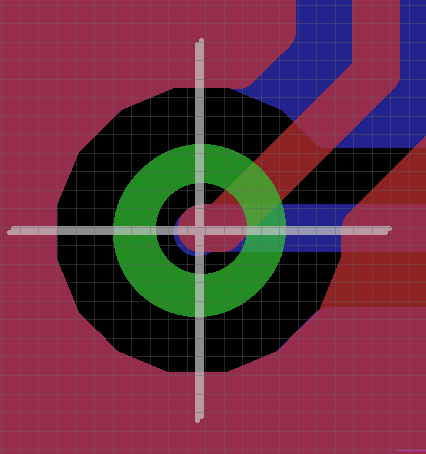
\includegraphics[width=0.6\textwidth]{img/DoubleDrillVia.png}
\end{center}
\caption{Overlapping via error}
\label{fig: doubledrill}
\end{figure}

\indent Once the errors were resolved, the designs were sent off to Advanced Circuits for fabrication. Final images of the RGBSaber\_control and RGBSaber\_periph layouts are shown in figures 2 and 3, below:
\begin{figure}[hbp]
\begin{center}
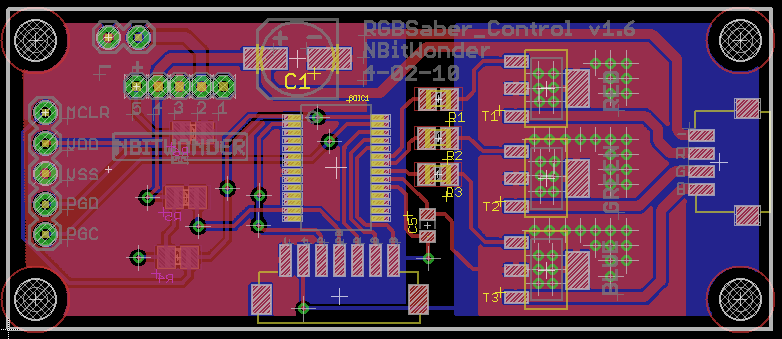
\includegraphics[width=0.6\textwidth]{img/RGBSaberControlv16LayoutComplete.png}
\end{center}
\caption{RGBSaber\_Control v1.6 Layout, Complete}
\label{fig: rgbsaber1.6controllay}
\end{figure}
%
\begin{figure}[hbp]
\begin{center}
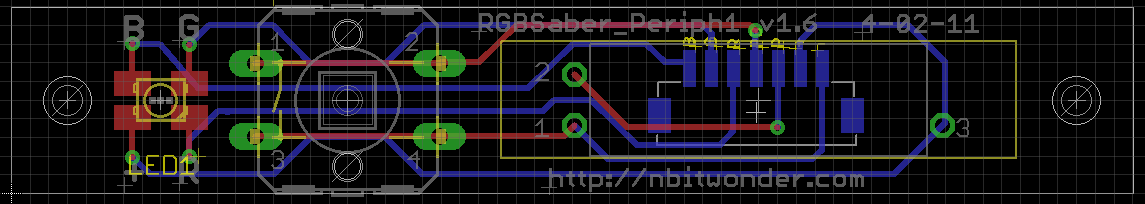
\includegraphics[width=0.6\textwidth]{img/RGBSaberPeriphv16LayoutComplete.png}
\end{center}
\caption{RGBSaber\_Periph v1.6 Layout Complete}
\label{fig: rgbsaber1.6periphlay}
\end{figure}
%
\end{nbentry}
%
% Sources Cited
% Add a section detailing all external source citations. The IEEE citation
%	style is recommended. For guidelines on using the IEEE citation style,
%	refer to
%   http://www.ieee.org/portal/cms_docs_iportals/iportals/publications/authors/transjnl/stylemanual.pdf

\end{document}
